\chapter{Описание алгоритма}
\label{cha:ch_2}

В данной главе будет описано обратимое и устойчивое к искажениям преобразование для построения спектрограммы из аудиосигнала.
Оно строится на основе операции многоканальной 1D свертки с заранее сформированным ядром, а также некоторой постобработки.

\section{Теоретическое обоснование алгоритма}
Напомним формулу 1D свертки. Пусть на входе есть двумерный массив данных $x: [L_{in} \times  C_{in}]$ 
и ядро свертки в виде массива $K: [C_{out} \times N \times C_{in}]$. Также задан шаг свертки $s$.
Тогда результат операции $y: [L_{out} \times C_{out}]$ рассчитывается по следующей формуле:
\begin{equation}
	y[i, c_{out}] = \sum_{j=0}^{N-1} \sum_{c_{in}=0}^{C_{in}-1} x[i \cdot s + j, c_{in}] \cdot K[c_{out}, j, c_{in}]
\end{equation}
\[i \in [0, L_{out}), \quad c_{out} \in [0, C_{out})\]
\[L_{out} = \lfloor(L_{in} - N) / s\rfloor + 1\]

\begin{figure}
  \centering
  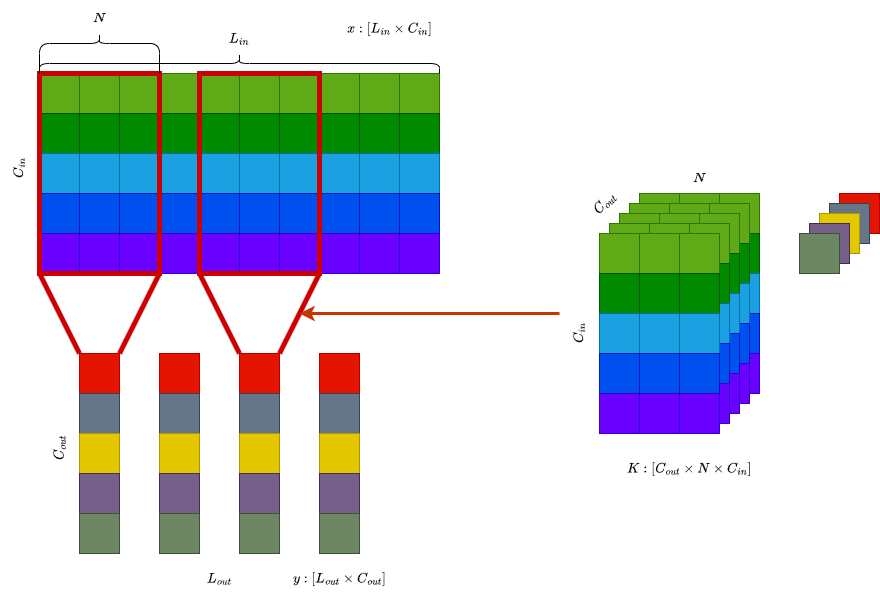
\includegraphics[width=0.9\linewidth]{figures/conv1d_drawio}
  \caption{Иллюстрации операции 1D свертки}
  \label{fig:conv1d_drawio}
\end{figure}

Каждый вектор $y_i: [1 \times C_{out}]$ можно рассматривать как матричное умножение вырезанного окна $x_i: [1 \times (N \cdot C_{in})]$ на матрицу $K^T: [(N \cdot C_{in}) \times C_{out}]$.

В случае, когда входным массивом является аудиосигнал, количество входных каналов $C_{in} = 1$, и можно несколько упростить формулу. 
\[x: [L_{in}], \quad K: [C_{out} \times N]\]
\begin{equation}
	y[i, c_{out}] = \sum_{j=0}^{N-1} x[i \cdot s + j] \cdot K[c_{out}, j]
\end{equation}


\textbf{Дискретное оконное преобразование Фурье (STFT)} можно посчитать через 1D свертку, если сформировать ядро $K_{\mathrm{stft}}: [N \times N]$ следующим образом:
\begin{equation}
	K_{\mathrm{stft}}[k, n] = e^{-i\pi \frac{(n - N/2) \cdot k}{N}} * w[n]
\end{equation}

\textbf{Дискретное вейвлет-преобразование (DWT)} на основе вейвлета Морле можно построить с помощью свертки с таким ядром:
\begin{equation}
	K_{\mathrm{dwt}}[k, n] = \psi^* \left(\frac{n - N/2}{a_0^k}\right)
\end{equation}
\[\psi(t) = e^{i\pi t} * e^{-\left(\frac{\pi t}{2\sigma}\right)^2}, \quad   a_0 \in (1, \infty)\]

На рисунке \ref{fig:stft_kernel} изображены ядра сверток для указанных преобразований, а также для преобразования, которое будет описано в данной работе.

\begin{figure}
  \centering
  \subfigure{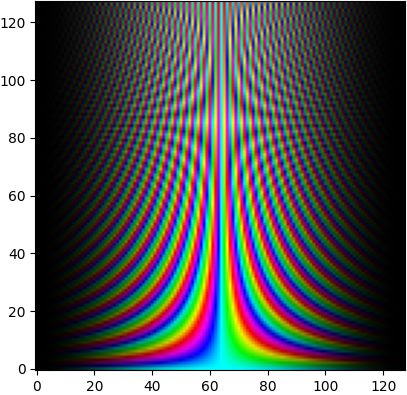
\includegraphics[width=0.3\textwidth]{figures/stft_kernel}} 
  \subfigure{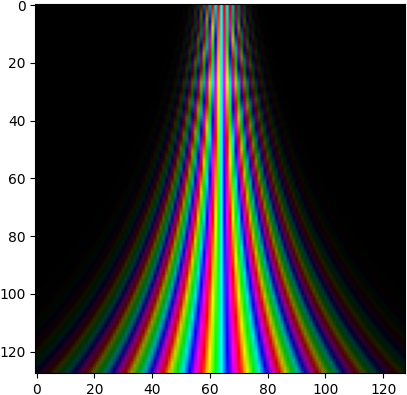
\includegraphics[width=0.3\textwidth]{figures/dwt_kernel}} 
  \subfigure{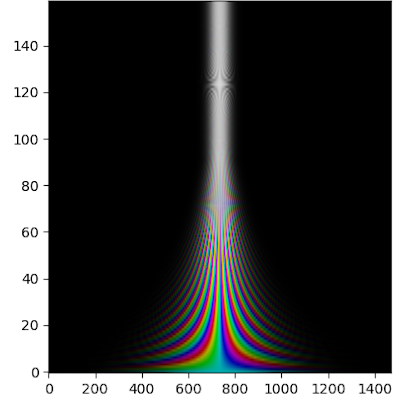
\includegraphics[width=0.3\textwidth]{figures/my_kernel}} 
  \caption{Ядро 1D свертки для STFT (1), вейвлет преобразования (2) и предлагаемого в работе преобразования (3)}
  \label{fig:stft_kernel}
\end{figure}


Теперь опишем процесс восстановления сигнала с помощью свертки, и при каких условиях он возможен.

Для начала рассмотрим преобразование, дискретное по частотам, но непрерывное по времени, 
представляющее собой свертку сигнала $x(t)$ с вейвлетом $\psi_m(t) = e^{2\pi i f_m t} \cdot w(t / \sigma_m)$.

\begin{equation}
  S_m(t)=\int \limits _{-\infty}^{+\infty}x(\tau)\,\psi_m(t - \tau)\,d\tau = \{x * \psi_m\}(t)
  \label{eq:conv_x_psi}
\end{equation}

Здесь и далее, запись $\{u*v\}(t)$ обозначает свертку в математическом смысле, которая определяется следующим образом:

\begin{equation}
  \{u*v\}(t)\triangleq \int \limits_{-\infty }^{\infty }u(\tau )v(t-\tau )\,d\tau = \int \limits_{-\infty }^{\infty }u(t-\tau )v(\tau )\,d\tau
\end{equation}

Полученная в равенстве \ref{eq:conv_x_psi} функция $S_m(t)$ представляет собой сигнал, ограниченный некоторой полосой частот, 
определяемой центральной частотой $f_m$ и спектральной шириной окна $\Delta f_m$.
Если посчитать спектр сигнала $S_m(t)$ с помощью преобразования Фурье, то, согласно теореме о свертке \cite{conv_theorem}, 
получим произведение спектра исходного сигнала $\mathcal{F}\{x(t)\}$ и спектра вейвлета $\mathcal{F}\{\psi_m^{*}(t)\}$.
Спектр вейвлета представляет собой спектр оконной функции, центр которого сдвинут к частоте $f_m$.

\begin{equation}
  \mathcal{F}\{S_m\}(f) = \mathcal{F}\{x\}(f) \cdot \mathcal{F}\{\psi_m\}(f)
\end{equation}

Если произвести снова свертку $S_m(t)$ с вейвлетом $\psi_m(t)$ в качестве этапа восстановления и посчитать спектр полученного сигнала, получим:

\begin{equation}
  \tilde{x}_m(t) = \{S_m * \psi_m\}(t) = \int \limits _{-\infty}^{+\infty} S_m(\tau)\,\psi_m(t - \tau)\,d\tau
\end{equation}
\begin{equation}
  \mathcal{F}\{\tilde{x}_m\} = \mathcal{F}\{S_m\} \cdot \mathcal{F}\{\psi_m\} = \mathcal{F}\{x\} \cdot (\mathcal{F}\{\psi_m\})^2
\end{equation}

Заметим, что спектр вейвлета является действительным в силу его симметричности $\psi(-t) = \psi^{*}(t)$, и равен спектру оконной функции, сдвинутым к центральной частоте $f_m$:
\begin{equation}
  \mathcal{F}\{\psi_m\}(f) = \mathcal{F}\{w(t/\sigma_m)\}(f - f_m) = \sigma_m \mathcal{F}\{w(t)\}((f - f_m) \sigma_m)
\end{equation}

При достаточно плотном перекрытии окон на оси частот, спектр исходного сигнала $\mathcal{F}\{x\}$ можно аналогично с методом, 
приведенным в Главе 1, разделе про восстановление сигнала от STFT (Равенство \ref{eq:weighted_sum_stft}), 
представить как взвешенную сумму:
\begin{equation}
  \mathcal{F}\{x\} = \frac{
    \sum \limits_m \mathcal{F}\{x\} \cdot (\mathcal{F}\{\psi_m\})^2
  }{
    \sum \limits_m (\mathcal{F}\{\psi_m\})^2
  } = 
  \frac{
    \sum \limits_m \mathcal{F}\{\tilde{x}_m\}
  }{
    \sum \limits_m (\mathcal{F}\{\psi_m\})^2
  }
\end{equation}

В силу линейности преобразования Фурье,

\begin{equation}
x(t) = K_{\psi} \sum \limits_m \tilde{x}_m(t) = K_{\psi} \sum \limits_m \{S_m * \psi_m\}(t)
\end{equation}

Отметим, что данная формула справедлива даже когда вейвлеты и ширина их окон не упорядочены по правилу $\psi_m = \psi(\frac{t}{a_0^m})$

\begin{markdown}
 - Оконное фурье через свертку
   - метод, окна, частоты, неопределенность
   - вычислительная сложность
 - оптимальный размер окна для конкретной шкалы частот
 - оптимальная форма окна для устойчивости к искажениям
 - Восстановление сигнала через свертку
 - Критерий восстановимости
 - восстановление сигнала с наложением
 - шкала амплитуд
 - выбор оптимальной шкалы частот
   - мел шкала
   - линейная шкала
   - комбинированная шкала
 - рекомендуемые значения параметров
 - связь количества частот и разрешения по времени
 - точность восстановления
 - избыточность информации в шумах
 - представление с сохранением фазы
 - представление с производной фазы
 - представление с магнитудой
 - Алгоритм Гриффина-Лима
  - адаптация
  - более точное восстановление при сохранении фазы
 - картинки
\end{markdown}

\section{Реализация алгоритма}
\begin{markdown}
 - описание алгоритма
   - подготовка ядра
     - шкала частот, df
	 - окна для каждой частоты
	 - Фурье базис с окнами, нормировка
	 - маска наложений
	 - ядро прямого прохода
	 - ядро обратного прохода
   - прямое преобразование
     - свертка
	 - преобразование фазы
	   - либо ничего
	   - либо производная фазы
	   - либо только магнитуда
	 - шкала амплитуд
   - обратное преобразование
     - шкала амплитуд
	 - восстановление фазы
	   - либо ничего
	   - либо интеграл (при этом накапливаются ошибки)
	   - либо GriffinLim
	 - свертка
 - код на Python
 - предложения для быстрой реализации
 - ускорение на GPU и TPU
 - визуализация спектрограмм
\end{markdown}

\section{Выводы по главе}
